\section{System Design}
Our setup consists of a Kinect camera rigidly aligned to an Oculus Rift HMD (Figure  \todo[inline]{Add picture of rft and kinect} ). The kinect acquires RGBD images which as used as input to the KinectFusion algorithm. Using the RGBD images, KinectFusion estimates the camera pose and uses this to integrate the current depthmap into the reconstruction. Virtual content is generated by animating a rigged model of a virtual character. The reconstruction is rendered from the viewpoint of the eyes. The virtual content is then composited onto this. If the virtual content is transformed using the same tracking as the reconstruction then it remains aligned to the environment.The combination of the reconstruction and virtual content is then rendered onto the HMD. Figure \todo[inline]{Add system overview figure} shows the System Overview. 
\missingfigure{System Overview}
\missingfigure{Picture of Rift}


\subsection{Environment Capture}
In order to capture the environment, we rely on the KinectFusion\cite{newcombe2011kinectfusion}  algorithm as our environment is static and we require the algorithm to be realtime. There are two main implementations of KinectFusion available. The Kinect Development Toolkit for Windows comes with an API to access KinectFusion. They do not provide source code but let the developer access KinectFusion in a limited matter. Also this version has only been demonstrated on small volumes and the tracking is not very stable when using large volumes with small voxel denisty. Given a camera pose and a camera matrix, the API allows the user to render the scene from that camera.\\
\begin{figure}[ht]
	\centering
	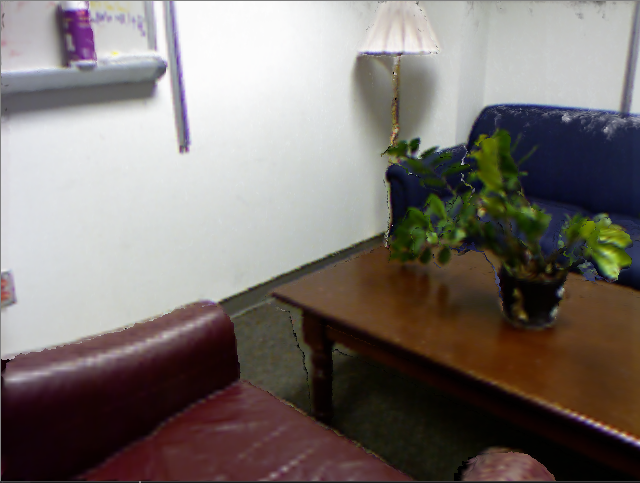
\includegraphics[width=3.0in]{images/scene2.png}
	\caption{A scene capture from Kinect}
	\label{fig:kinectFusionOut}
\end{figure}
The other popular implementation is KinFu that comes with PCL. This contains extensions on KinectFusion that enable it to work in large areas. It does so by decomposing the environment into chunks that can be uploaded to the GPU. This allows it to reconstruct a large volume while maintaining a high voxel density.This results in more robust tracking.  


\subsection{Generate Virtual Content}

\subsection{Composit Real and Virtuals}

\subsection{Tracking}

\subsection{Display on HMD}